\chapter{Metodologia}

Essa seção de metodologia é analoga à etapa de Rever ou produzir modelos de Processos da fase de Definição do GQM.


Para a execução deste plano, decidiu-se uma metodologia de trabalho na qual teremos vários encontros com os clientes responsáveis pelas entregas de dados, vulgo grupos de Engenharia de Requisitos, pois por ter um convívio diário no mesmo ambiente facilitará a coleta de dados.

Planeja-se fazer encontros semanais com os responsáveis pela coleta das métricas para poder obter estes dados e continuar a análise do trabalho. 

Os dados serão anotados em uma planilha do Google Drive, separados em abas por equipe, para ter um controle maior e poder utilizar cálculos automatizados, que a própria ferramenta oferece.
	
O processo de medição e análise ocorrerá em iterações de uma semana, na qual teremos ao seu início a coleta das métricas, análise destas através deste plano e ao final de cada iteração, uma conclusão ou atualização da conclusão das métricas, e ao final de todas as iterações, a conclusão final do plano.


\begin{figure}[H]
  \center
  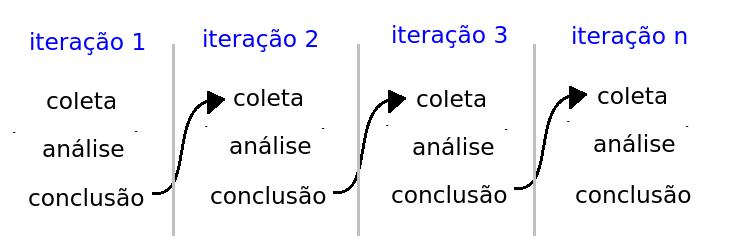
\includegraphics[width=0.8\textwidth]{figuras/iteracoes.png}
  \caption{Iterações}
  \label{fig:iteracoes}
\end{figure}